\begin{tikzpicture}
    %\draw (0, 0) rectangle (14, 6);
    \node at (3, 2) {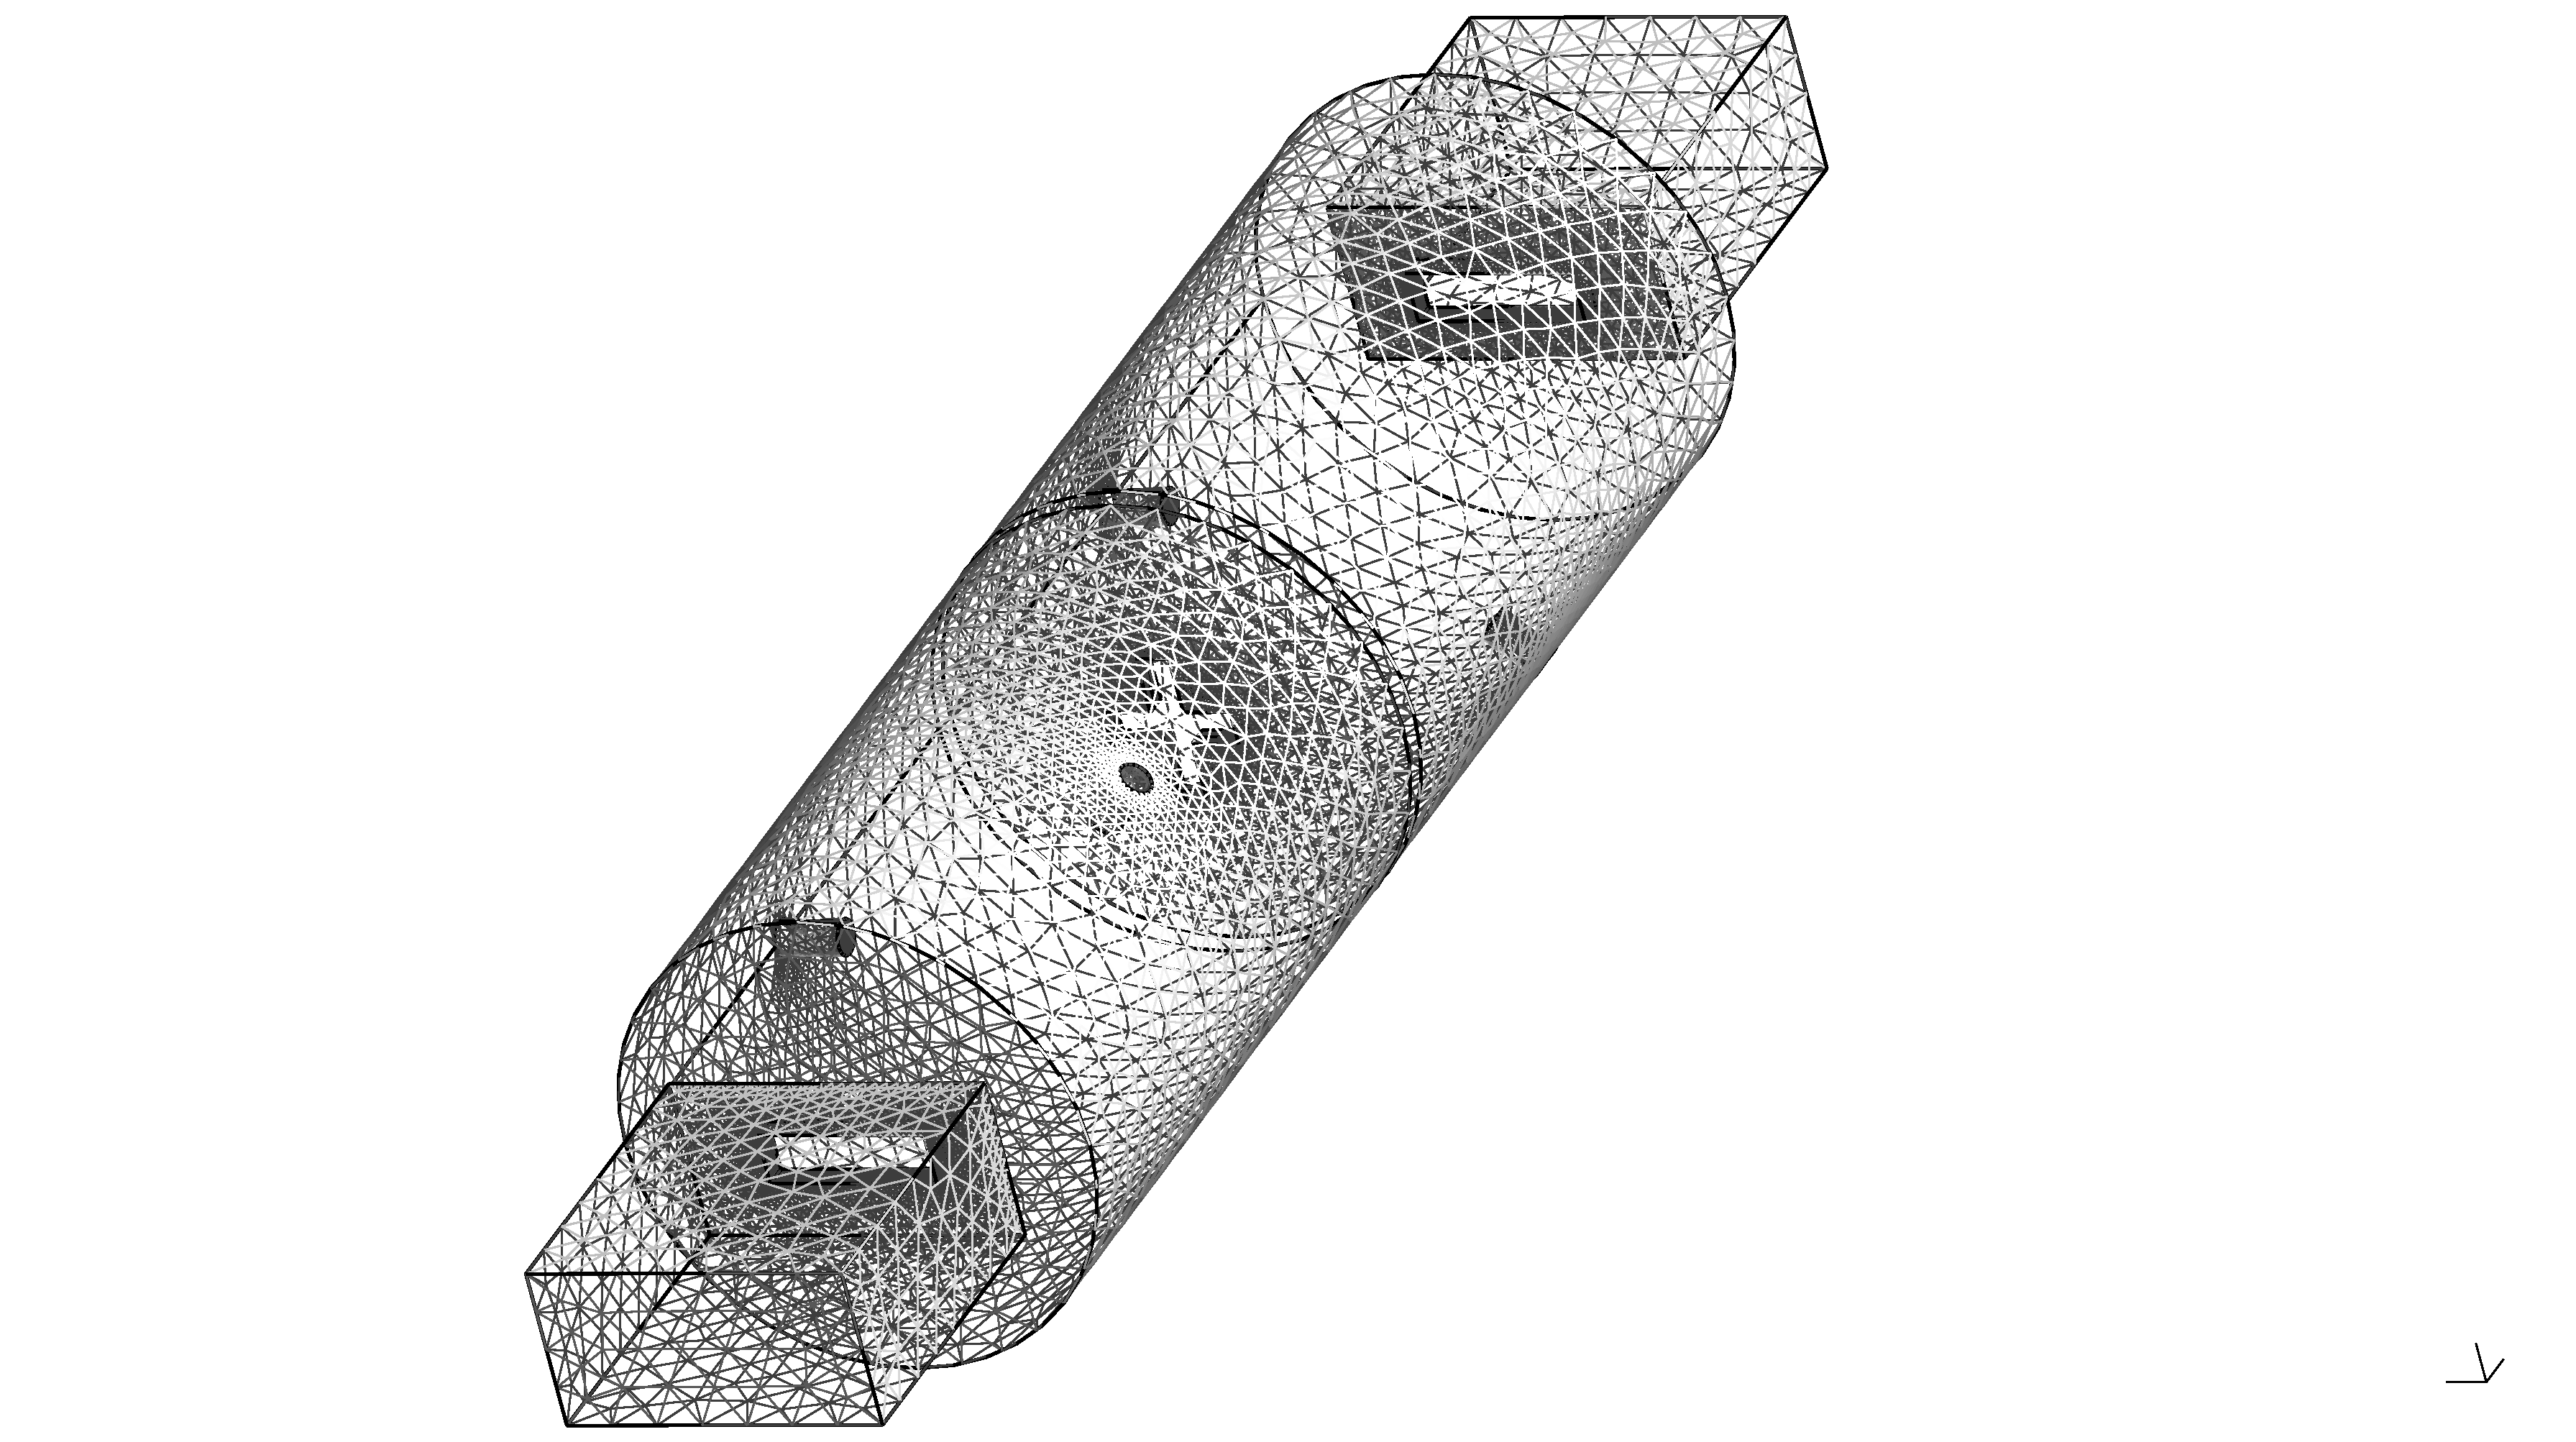
\includegraphics[scale=0.18, trim=12cm 0.2cm 15cm 0.2cm, clip]{figures/DMCWF_surfacemesh.pdf}};
    %\node at (9.4, 2.5) {\includegraphics[scale=0.087]{DMCWF_top.pdf}};
    \draw[thick, fill=black!5!white] (5.65, 1.9) rectangle (6.9, 3.1);
    \draw[thick, fill=black!5!white] (7, 1.6) rectangle (9.75, 3.4);
    \draw[thick, fill=black!5!white] (9.85, 1.6) rectangle (12.65, 3.4);
    \draw[thick, fill=black!5!white] (12.75, 1.9) rectangle (14, 3.1);
    \draw[thick] (6.9, 2.15) to (7, 2.15);
    \draw[thick] (6.9, 2.85) to (7, 2.85);
    \draw[thick] (12.65, 2.15) to (12.75, 2.15);
    \draw[thick] (12.65, 2.85) to (12.75, 2.85);
    \draw[thick] (9.75, 2.25) to (9.85, 2.25);
    \draw[thick] (9.75, 2.75) to (9.85, 2.75);
    \draw[thick] (8.37, 1.85) ellipse (0.07 and 0.04);
    \draw[thick, opacity=0.2] (11.25, 1.85) ellipse (0.07 and 0.04);
    \draw[thick] (8.29, 3.375) to (8.44, 3.375);
    \draw[thick] (11.17, 3.375) to (11.33, 3.375);

    \draw[<->] (7, 3.6) -- (9.75, 3.6) node [midway, above] {$L_C$};
    \draw[<->] (5.65, 3.3) -- (6.9, 3.3) node [midway, above] {$L_B$};
    \draw[<->] (5.45, 3.1) -- (5.45, 1.9) node [midway, left] {$W_B$};
    \draw[<->] (7.8, 1.7) -- (7.8, 3.3) node [midway, left] {$D_C$};

    \begin{scope}[shift={(0, -0.5)}]

        \draw[thick, fill=black!5!white] (6.5, 0) circle (1);
        \draw[thick, fill=black!10!white] (5.8, -0.35) rectangle (7.2, 0.35);
        \draw[thick, fill=white] (6.1, -0.083) rectangle (6.9, 0.083);

        \draw[dashed] (6.1, 0.083) to (6.1, 1.25);
        \draw[dashed] (6.9, 0.083) to (6.9, 1.25);
        \draw[<->] (6.1, 1.15) -- (6.9, 1.15) node [midway, above] {$W_S$};
        \draw[dashed] (6.1, 0.083) to (5.2, 0.083);
        \draw[dashed] (6.1, -0.083) to (5.2, -0.083);
        \draw[<->] (5.3, -0.083) -- (5.3, 0.083) node [midway, left] {$H_S$};
        \draw[dashed] (7.2, -0.35) to (7.7, -0.35);
        \draw[dashed] (7.2, 0.35) to (7.7, 0.35);
        \draw[<->] (7.6, -0.35) -- (7.6, 0.35) node [midway, right] {$H_B$};

    \end{scope}

    \begin{scope}[shift={(0.05, -0.5)}]

        \draw[thick, fill=black!5!white] (9.76, 0) circle (1);
        \draw[thick, fill=white] (9.68, -0.35) to (9.84, -0.35) to (9.84, -0.08) to (10.06, -0.08)
                        to (10.06, 0.08) to (9.84, 0.08) to (9.84, 0.35) to (9.68, 0.35)
                        to (9.68, 0.08) to (9.46, 0.08) to (9.46, -0.08) to (9.68, -0.08)
                        to cycle;


        \draw[dashed] (9.84, 0.35) to (9.84, 1.25);
        \draw[dashed] (9.68, 0.35) to (9.68, 1.25);
        \draw[<->] (9.68, 1.15) -- (9.84, 1.15) node [midway, above] {$W_A$};
        
        \draw[dashed] (9.68, -0.35) to (9.68, -1.25);
        \draw[dashed] (9.46, -0.083) to (9.46, -1.25);
        \draw[<->] (9.46, -1.15) -- (9.68, -1.15) node [midway, below] {$L_A$};

        %\draw[dashed] (9.46, -0.083) to (8.5, -0.083);
        %\draw[dashed] (9.46, 0.083) to (8.5, 0.083);
        %\draw[<->] (8.6, -0.083) -- (8.6, 0.083) node [midway, left] {$c$};
        
        \draw[dashed] (9.84, 0.35) to (11, 0.35);
        \draw[dashed] (10.06, 0.083) to (11, 0.083);
        \draw[<->] (10.9, 0.083) -- (10.9, 0.35) node [midway, right] {$H_A$};

    \end{scope}
\end{tikzpicture}